\section{Quaternioni}
\label{ch1:quaternions}
\indent

Quaternionii au fost descoperiți de Sir William Rowan Hamilton in secolul al
XIX-lea. Acesta căuta un mod de a reprezenta numerele complexe in dimensiuni
superioare. De la descoperirea lor, matematicienii au arătat că quaternionii pot
fi utilizați pentru a roti puncte în jurul unor axe arbitrare.
Quaternionii au o serie de avantaje față de matrici. De exemplu, pentru
stocarea unui quaternion sunt nevoie doar de patru componente, concatenarea lor
implică mai puține operații aritmetice și sunt mai ușor de interpolat pentru a
produce animații. Utilizarea lor în grafica 3D a fost pionierată de
\todo{inserat referinta} Shoemake.

\todo{Schimbat titlul}
\subsection{Proprietățile quaternionilor}
\label{ch1:quaternions:properties}
\indent

Mulțimea quaternionilor, cunoscută în matematică sub denumirea de \textit{inelul
quaternionilor Hamiltonieni} și notată cu $\mathbb{H}$ poate fi văzută ca
un spațiu vectorial patru dimensional, ale cărui elemente sunt tuple de 4
numere reale, de forma 
\begin{equation}
q = \langle w, x, y, z\rangle = w + x\mathit{i} + y\mathit{j} + z\mathit{k}.
\end{equation}
Un quaternion mai poate fi scris și ca 
\begin{equation}
q = \lbrack s, v \rbrack
\end{equation} unde s este partea scalară, iar v este partea vectorială.
Hamilton a numit quaternionii ai căror componentă scalară este egală cu zero
\textit{quaternioni puri}.
%\newpage
\begin{lstlisting}[
    title={Cod C++}, 
    xleftmargin=2pt,
    abovecaptionskip=2pt,
    belowcaptionskip=2pt,
    frame=single
    ]
template<typename real_t>
class quaternion {
public :
    union {
        struct {
            real_t w_;
            real_t x_;
            real_t y_;
            real_t z_;
        };
        real_t elements_[4];
    };

    quaternion();
    quaternion(real_t w, real_t x, real_t y, real_t z);
    quaternion(const real_t* init_data);
    quaternion(const vector3<real_t>&, real_t w = real_t(0));
    ...
};
\end{lstlisting}

\subsection{Adunarea quaternionilor}
\label{ch1:quaternions:addition}
Quaternionii se adună și se scad pe componente, ca și vectorii.
Fiind dați doi quaternioni, $q_1 \text{ și } q_2$, suma lor este quaternionul
\begin{equation}
q = q_1 + q_2 = \lbrack s_1 + s_2, v_1 + v_2 \rbrack,
\end{equation} sau echivalent
\begin{equation}
q = q_1 + q_2 = \langle w_1 + w_2, \quad (x_1 + x_2)i, \quad (y_1 + y_2)j, 
\quad (z_1 + z_2)k \rangle.
\end{equation}

\begin{lstlisting}[
    title={Cod C++}, 
    xleftmargin=2pt,
    abovecaptionskip=2pt,
    belowcaptionskip=2pt,
    frame=single
    ]
template<typename real_t>
gfx::quaternion<real_t>&
gfx::quaternion<real_t>::operator +=(
    const gfx::quaternion<real_t>& rhs
    )
{
    w_ += rhs.w_; x_ += rhs.x_; y_ += rhs.y_; z_ += rhs.z_;
    return *this;
}

\end{lstlisting}

\noindent
Proprietățile adunării quaternionilor :
\begin{enumerate}
    \item Adunarea este comutativă : 
    $q_1 + q_2 = q_2 + q_1, \quad \forall q_1, q_2 \in \mathbb{H}$
    \item Adunarea este asociativă :
    $(q_1 + q_2) + q_3 = q_1 + (q_2 + q_3), \quad \forall q_1, q_2, q_3
    \in \mathbb{H}$
    \item Element neutru : $\exists q' = \langle 0, 0, 0, 0 \rangle \in 
    \mathbb{H} \text{ a. î. } q + q' = q' + q = q, \quad \forall q \in
    \mathbb{H}$ 
    \item Orice quaternion are un opus : $\forall q \in \mathbb{H} \quad
    \exists q' = (-q) \in \mathbb{H} \quad \text{ a.î. } q + q' = q' + q = 
    \langle 0, 0, 0, 0 \rangle$
\end{enumerate}

\subsection{Opusul unui quaternion}
Opusul unui quaternion are o proprietate interesantă. Deși la prima vedere s-ar
părea că el anulează rotația aplicată de quaternionul original, 
rotația prin opusul quaternionului se efectuează în jurul axei negative. 
Rezultatul este că un vector rotit printr-un quaternion sau opusul acelui 
quaternion ajunge tot în aceeași poziție. Diferența este că în timp ce 
quaternionul original aplică o rotație de $\theta$ radiani în jurul
unei axe $\mathbf{\hat{r}}$, opusul său aplică o rotație de $2\pi - \theta$
radiani în jurul axei $\mathbf{-\hat{r}}$.
\begin{figure}
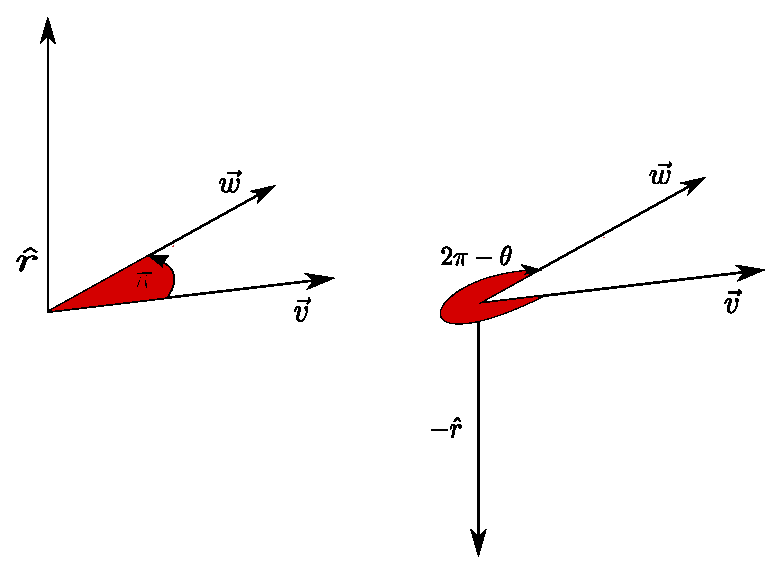
\includegraphics{quaternion_rotation.eps}
\caption{Rotirea unui vector printr-un quaternion $q$ (stânga) și prin opusul său
$-q$ (dreapta).}
\label{fig:quat_rotation}
\end{figure}

\subsection{Magnitudinea unui quaternion}
\label{ch1:quaternions:magnitude}
Similar cu vectorii, magnitudinea unui quaternion este dată de formula
\begin{equation}
\Vert q \Vert = \sqrt{w^2 + x^2 + y^2 + z^2}.
\end{equation}
Un quaternion care are o magnitudine de unu se spune că este un
\textit{quaternion unitate}. Componentele unui quaternion unitate verifică
relația
\begin{equation}
w^2 + v \cdot v = 1.
\end{equation}
Similar vectorilor, un quaternion cu o magnitudine
non-zero poate fi adus la lungime unitate prin operația de normalizare, adică
\begin{equation}
\hat{q} = \frac{q}{\Vert q \Vert}.
\end{equation}
Fie q și r quaternioni din $\mathbb{H}$. Se verifică următoarele relații :
\begin{enumerate}
    \item $\Vert q \Vert ^ 2 = w^2 + v \cdot v$
    \item $\Vert q \Vert = 0 \iff q = \langle 0, 0, 0, 0 \rangle$
    \item $\Vert \mathit{a}q \Vert = \vert \mathit{a} \vert \Vert q \Vert$
    \item $\Vert q + r \Vert \leq \Vert q \Vert + \Vert r \Vert$
\end{enumerate}

\begin{lstlisting}[
    title={Cod C++}, 
    xleftmargin=2pt,
    abovecaptionskip=2pt,
    belowcaptionskip=2pt,
    frame=single
    ]
template<typename real_t>
inline real_t gfx::quaternion<real_t>::length_squared() const {
    return w_ * w_ + x_ * x_ + y_ * y_ + z_ * z_;
}

template<typename real_t>
inline real_t gfx::quaternion<real_t>::magnitude() const {
    return std::sqrt(length_squared());
}

template<typename real_t>
gfx::quaternion<real_t>& gfx::quaternion<real_t>::normalize() {
    const real_t len_sq = length_squared();
    if (math::operands_eq(real_t(0), len_sq))
        return make_zero();

    const real_t scale_factor = real_t(1) / len_sq;
    w_ *= scale_factor; 
    x_ *= scale_factor; 
    y_ *= scale_factor; 
    z_ *= scale_factor;
    return *this;
}
\end{lstlisting}

\subsection{Produs scalar}
\label{ch1:quaternions:scalar_product}
Produsul scalar a doi quaternioni este similar cu produsul scalar a doi vectori,
fiind suma produselor componentelor celor doi operanzi. Fie $q_{1} \text{ și }
q_{2}$ doi quaternioni din $\mathbb{H}$. Atunci produsul scalar al lor este dat de
formula
\begin{equation}
q_{1} \cdot q_{2} = \sum_{i = 1}^{4} q_{1i}q_{2i} 
\end{equation} sau echivalent
\begin{equation}
q_{1} \cdot q_{2} = w_{1}w_{2} + x_{1}x_{2} + y_{1}y_{2} + z_{1}z_{2}.
\end{equation}
Produsul scalar mai verifică și următoarele relații :
\begin{enumerate}
\item $q_1 \cdot q_2 = q_2 \cdot q_1$
\item $q \cdot q = \Vert q \Vert ^ 2$
\item $q_1 \cdot q_2 = 1 \Rightarrow q_1 \perp q_2$
\item $(\mathit{a}q_1) \cdot q_2 = \mathit{a}(q_1 \cdot q_2)$
\end{enumerate}
\todo{Verificat chestia asta din VanVerth}
Produsul scalar a doi quaternioni dă o masură a diferenței dintre rotațiile
aplicate de cei doi quaternioni. Presupunând că quaternionii sunt normalizați,
când produsul ia valori apropiate de 1 sau -1, cei doi quaternioni aplică 
rotații similare. În consecință, quaternioni normalizați al căror produs ia
valori apropiate de 0 produc rotații  forte diferite. Iată și implementarea
produsului scalar în cod :

\begin{lstlisting}[
    title={Cod C++}, 
    xleftmargin=2pt,
    abovecaptionskip=2pt,
    belowcaptionskip=2pt,
    frame=single
    ]
template<typename real_t>
inline
real_t
gfx::dot_product(
    const gfx::quaternion<real_t>& lhs, 
    const gfx::quaternion<real_t>& rhs
    )
{
    return lhs.x_ * rhs.x_ + lhs.y_ * rhs.y_ 
           + lhs.z_ * rhs.z_ + lhs.w_ * rhs.w_;
}
\end{lstlisting}

\subsection{Conversia între formate}
Dându-se un unghi de rotație $\theta$ și o axă de rotație $\hat{r}$, conversia de 
la formatul axă-unghi la quaternion este dată de formula :
\begin{equation}
q = \left\lbrack \cos\left(\frac{\theta}{2}\right), 
    \hat{r}\sin\left(\frac{\theta}{2}\right) \right\rbrack 
\end{equation}
Pentru a converti de la quaternion (normalizat) la format axă-unghi se 
determină mai intâi unghiul de rotație :
\[
w = \cos\left(\frac{\theta}{2}\right) \rightarrow \theta = 2\arccos\left(w\right)
\]
Cum pentru un quaternion normalizat avem $w^2 + v \cdot v = 1$, rezultă că
$\Vert v \Vert = \sqrt{1 - w^2}$. Atunci, vectorul care dă axa de rotație se 
determină astfel :
\[
\hat{r} = \frac{v}{\Vert v \Vert}
\]

Matricea pătratică de ordinul trei care aplică aceeași rotație ca și un 
quaternion $q$ este dată de formula :
\begin{equation}
\mathbf{M}_{q} = 
\begin{bmatrix}
1 - 2y^2 - 2z^2 & 2xy - 2wz         & 2xz + 2wy \\
2xy + 2wz       & 1 - 2x^2 - 2z^2   & 2yz - 2wx \\
2xz - 2wy       & 2yz + 2wx         & 1 - 2x^2 - 2y^2
\end{bmatrix}
\end{equation}
Dacă quaternionul nu este normalizat, matricea trebuie scalată cu
\[
\frac{1}{w^2 + x^2 + y^2 + z^2}
\]
Codul care realizează conversia de la quaternion la matrice de rotație este
implementat pe baza articolelor \cite{Shoemake95} și \cite{Shoemake89} :
\begin{lstlisting}[
    title={Cod C++}, 
    xleftmargin=2pt,
    abovecaptionskip=2pt,
    belowcaptionskip=2pt,
    frame=single
]
template<typename real_t>
gfx::quaternion<real_t>&
gfx::quaternion<real_t>::to_rotation_matrix(
    gfx::matrix_3X3<real_t>* mtx
    ) const
{
    real_t s, xs, ys, zs, wx, wy, wz, xx, xy, xz, yy, yz, zz;

    s = 2 / length_squared();

    xs = s * x_;
    ys = s * y_;
    zs = s * z_;

    wx = w_ * xs;
    wy = w_ * ys;
    wz = w_ * zs;

    xx = x_ * xs;
    xy = x_ * ys;
    xz = x_ * zs;

    yy = y_ * ys;
    yz = y_ * zs;

    zz = z_ * zs;

    mtx->a11_ = real_t(1) - (yy + zz);
    mtx->a12_ = xy - wz;
    mtx->a13_ = xz + wy;

    mtx->a21_ = xy + wz;
    mtx->a22_ = real_t(1) - (xx + zz);
    mtx->a23_ = yz - wx;

    mtx->a31_ = xz - wy;
    mtx->a32_ = yz + wx;
    mtx->a33_ = real_t(1) - (xx + yy);

    return *this;
}
\end{lstlisting}

\subsection{Înmulțirea quaternionilor}
\label{ch1:quaternions:multiplication}
Fiind dați doi quaternioni
\begin{IEEEeqnarray*}{rCl}
q_{1} = w_{1} + v_{1} = w_{1} + x_{1}\mathit{i} + y_{1}\mathit{j} 
                         + z_{1}\mathit{k},\\
q_{2} = w_{2} + v_{2} = w_{2} + x_{2}\mathit{i} + y_{2}\mathit{j}
                        + z_{2}\mathit{k},
\end{IEEEeqnarray*}
produsul lor este dat de
\begin{IEEEeqnarray*}{rCl}
q_{1}q_{2} = (w_{1}w_{2} - x_{1}x_{2} - y_{1}y_{2} - z_{1}z_{2})\\
+ (w_{1}x_{2} + x_{1}w_{2} + y_{2}z_{2} - z_{1}y_{2})\mathit{i}\\
+ (w_{1}y_{2} - x_{1}z_{2} + y_{1}w_{2} + z_{1}x_{2})\mathit{j}\\
+ (w_{1}z_{2} + x_{1}y_{2} - y_{1}x_{2} + z_{1}w_{2})\mathit{k}\IEEEyesnumber
\end{IEEEeqnarray*} sau echivalent
\begin{equation}
q_{1}q_{2} = w_{1}w_{2} - v_{1} \cdot v_{2} + w_{1}v_{2} + w_{2}v_{1} +
v_{1} \times v_{2}.
\end{equation}
Se poate observa că produsul a doi quaternioni este necomutativ, deoarece
conține un produs vectorial în componența sa.
Proprietățile înmulțirii quaternionilor.
\begin{enumerate}
    \item $q_{1}q_{2} \neq q_{2}q_{1}, \quad \forall q_{1}, q_{2} \in
    \mathbb{H}$
    \item $q_{1}(q_{2}q_{3}) = (q_{1}q_{2})q_{3}, \quad \forall q_{1}, q_{2},
    q_{3} \in \mathbb{H}$
    \item $\exists q_{I} \in \mathbb{H} \text{ a.î. } qq_{I} = q_{I}q = q,
    \forall q \in \mathbb{H}$
    \item $\exists q^{-1} \in \mathbb{H} \text{ a.î. } qq^{-1} = q^{-1}q =
    q_{I}, \quad \forall q \in \mathbb{H}$
    \item $q_{1}(q_{2} + q_{3}) = q_{1}q_{2} + q_{1}q_{3} \quad \forall q_{1},
    q_{2}, q_{3} \in \mathbb{H}$
\end{enumerate}

\begin{lstlisting}[
    title={Cod C++}, 
    xleftmargin=2pt,
    abovecaptionskip=2pt,
    belowcaptionskip=2pt,
    frame=single
]
template<typename real_t>
gfx::quaternion<real_t>
gfx::operator*(
    const gfx::quaternion<real_t>& lhs, 
    const gfx::quaternion<real_t>& rhs
    )
{
    vector3<real_t> v1(lhs.x_, lhs.y_, lhs.z_);
    vector3<real_t> v2(rhs.x_, rhs.y_, rhs.z_);

    quaternion<real_t> result;
    result.w_ = lhs.w_ * rhs.w_ - dot_product(v1, v2);
    result.x_ = lhs.w_ * rhs.x_ + rhs.w_ * lhs.x_ 
                + lhs.y_ * rhs.z_ - lhs.z_ * rhs.y_;
    result.y_ = lhs.w_ * rhs.y_ + rhs.w_ * lhs.y_ 
                + lhs.z_ * rhs.x_ - lhs.x_ * rhs.z_;
    result.z_ = lhs.w_ * rhs.z_ + rhs.w_ * lhs.z_ 
                + lhs.x_ * rhs.y_ - lhs.y_ * rhs.x_;
    return result;
}
\end{lstlisting}
Ca și în cazul matricilor, concatenarea mai multor quaternioni va rezulta în 
cumularea rotațiilor efectuate de quaternionii respectivi.

\subsection{Conjugata unui quaternion}
\label{ch1:quaternions:conjugate}
Ca și numerele complexe, quaternionii au conjugate.
Dacă $q = s + v$ este un quaternion din $\mathbb{H}$, atunci conjugatul său este
quaternionul
\begin{equation}
\bar{q} = s - v = s - (x\mathit{i} + y\mathit{j} + z\mathit{k}).
\end{equation}
Dacă efectuăm produsul între un quaternion și conjugatul său, obținem :
\[
q\bar{q} = w\bar{w} - v \cdot \bar{v} + w\bar{v} + \bar{w}v + v \times \bar{v}.
\]
Cum $v = -\bar{v} \text{ și } w = \bar{w}$ rezultă că $q\bar{q} = w^2 +
v\cdot v$, adică există identitatea : 
\begin{equation}
q\bar{q} = \bar{q}q = q \cdot q = \Vert q \Vert ^ 2.
\end{equation}

\subsection{Inversa unui quaternion}
\label{ch1:quaternions:inverse}
Inversul unui quaternion non-zero $q \in \mathbb{H}$ este quaternionul dat de 
formula
\begin{equation}
\label{eq:quat_inverse}
q^{-1} = \frac{\bar{q}}{\Vert q \Vert ^ 2}.
\end{equation}
Dacă q este un \textit{quaternion de magnitudine unitate}, formula
\eqref{eq:quat_inverse} poate fi redusă la
\begin{equation}
q^{-1} = \bar{q}.
\end{equation}

\begin{figure}
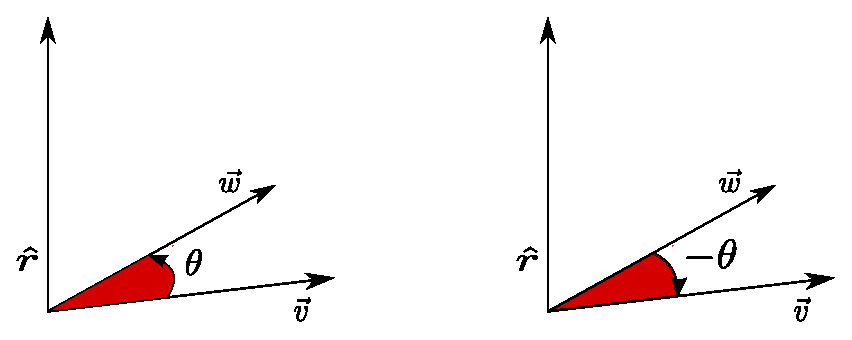
\includegraphics{quaternion_inverted.eps}
\caption{Relația dintre un quaternion și inversul său.}
\end{figure}

Practic, dacă un quaternion $q$ efectuează o rotație de $\theta$ radiani, 
în sens trigonometric (sensul invers acelor de ceasornic), în jurul unei axe 
$\hat{r}$, inversul său efectuează o rotație de $\theta$ radiani, în jurul 
aceleiași axe $\hat{r}$, dar în sensul opus sensului trigonometric (sensul 
acelor de ceasornic).

\begin{lstlisting}[
    title={Cod C++}, 
    xleftmargin=2pt,
    abovecaptionskip=2pt,
    belowcaptionskip=2pt,
    frame=single
    ]
template<typename real_t>
gfx::quaternion<real_t>& gfx::quaternion<real_t>::invert() {
    const real_t len_sq = length_squared();
    if (math::operands_eq(real_t(0), len_sq)) {
        return make_identity();
    }

    const real_t scale_factor = 1 / len_sq;
    w_ *= scale_factor;
    x_ = (-x_ * scale_factor);
    y_ = (-y_ * scale_factor);
    z_ = (-z_ * scale_factor);

    return *this;
}
\end{lstlisting}


\subsection{Rotirea vectorilor}
\label{ch1:quaternions:vector_rotation}
